% !TEX root = main.tex
% \renewcommand{\MintedPygmentize}{/alaink/miniconda3/bin/pygmantize}
\documentclass{article}
\usepackage{algorithm}
\usepackage{algpseudocode}
\usepackage{graphicx}
\usepackage[a4paper,top=2cm,bottom=2cm,left=2cm,right=2cm]{geometry}
\usepackage{setspace}

\begin{document}
\doublespacing
\title{Parallel lifting algorithms for phason strain calculations}
\maketitle
Alain Kadar - Glotzer Group and Kotov Lab

\vspace{1cm}

\textbf{In the materials science community, phason strain calculations are an important part of assessing the structural quality of quasicrystals. The structure of a quasicrystal is well represented by a collection of points. A crucial component of the phason strain calculation amounts to determining how these points can be reached from a given origin point by some integer combination of basis vectors. This process is called "lifting". Currently, there exists no rapid and scaleable implementation of a lifting algorithm. In this report, we assess the effectiveness of several parallel computing techniques for reducing lifting times. Namely, we demonstrate that parallelizing searches of the neighbor list reduces the time taken to run the algorithm and that the attained speedup increases with system size. We show the same is true for parallelization of the visited array search and so nest these parallelizations using OpenMP. We implement a parallelized queue and kernelize multiplication of the basis and difference matrices on the GPU, using CUDA. However, we find that these techniques incur a computational overhead which negates the benefits of parallelization for the size of systems we are dealing with. The fact that speedup increases with system size, motivates the simulation of larger systems, which is already underway as part of the Glotzer group's future work.}


\section{Lifting procedure}
Lifting requires a set of points and basis vectors. For quasicrystals, the number of basis vectors, M, is always larger than the number of dimensions, R, in which the points are embedded. For example, Figure \ref{fig:schematic} shows a collection of points in 3 dimensions (although the third is trivial), with 5 basis vectors. In the context of this formalism, quasicrystals can be thought of as being periodic in a higher dimensional space (in this case, a 5 dimensional hyperspace). The large points are simply reference points and not included in any lifting analysis. The basis vectors are stored in $\mathbf{Q}$. When every point in a system may be reached by the basis vectors, the system is said to be "perfect". Every point that cannot be reached is a defect.

\begin{figure}[htp!]
    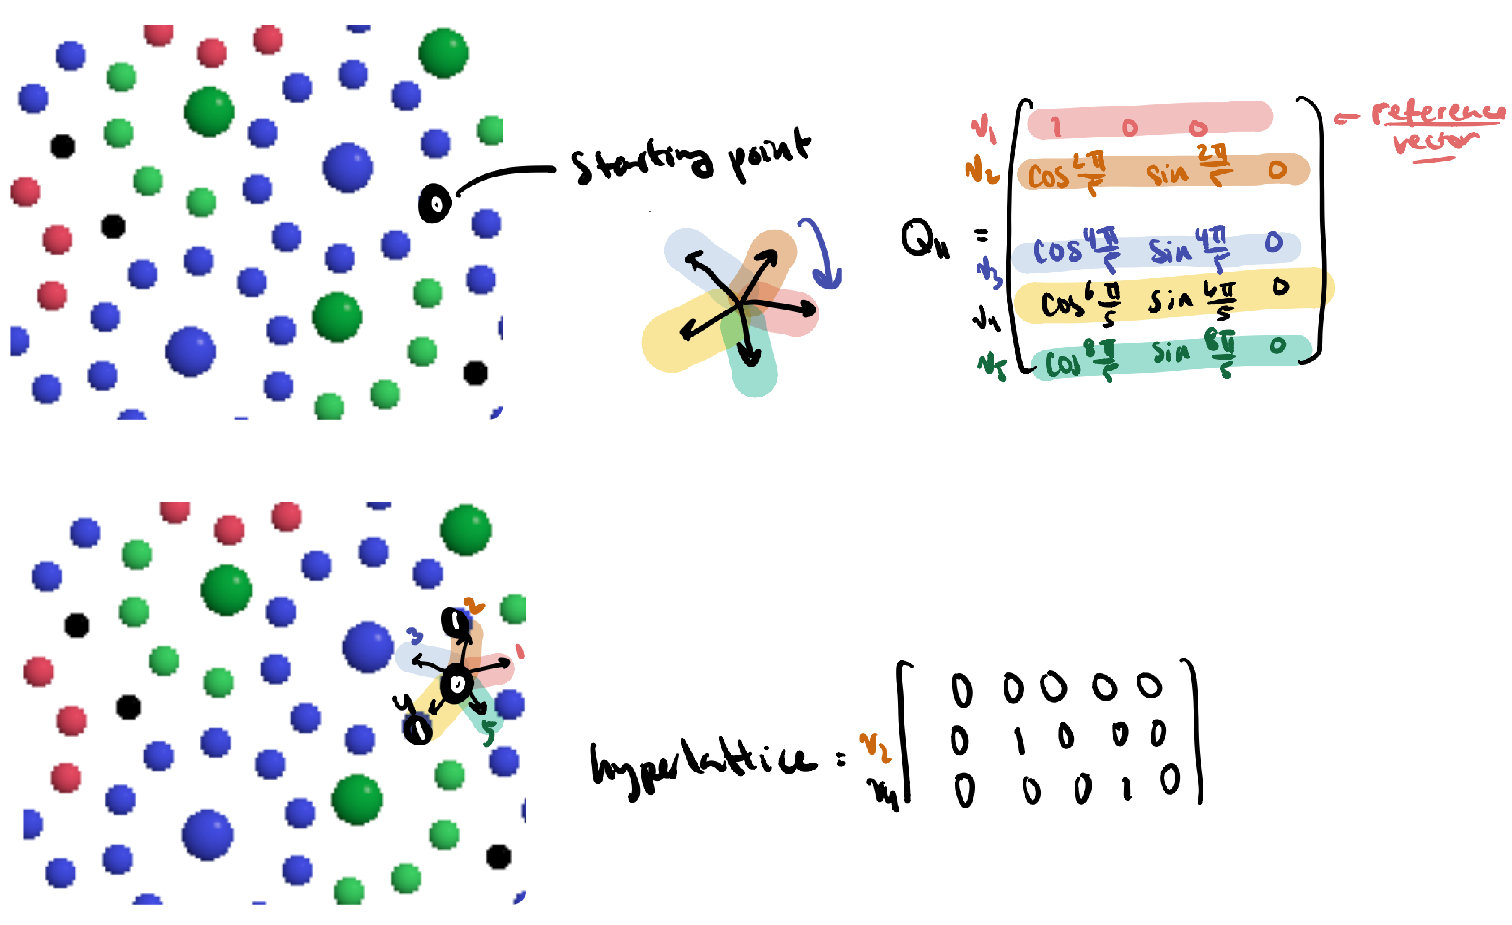
\includegraphics[scale=0.8]{schematic.png}
    \caption{Schematic for the lifting procedure. The upper panel shows which particle is chosen as the origin, and the basis vectors. The matrix, $\mathbf{Q}$ is simply where the basis vectors are stored. The lower panel shows that 2 unvisited neighbors of the origin were identified as being in alignment with one of the basis vectors. The hyperlattice matrix is updated accordingly. Figure adapted from a schematic by Kelly Wang of Glotzer group.}
    \label{fig:schematic}
    \centering
\end{figure}

The inputs for lifting include the positions of every point and the basis set of vectors. With this, an origin particle is selected and its neighbor's determined. A vector connecting a reference particle with its neighbor is a "positional difference vector". All neighbors that can be reached by a vector from the basis set are retained, and the particular basis vector by which they can be reached is noted. To account for thermal noise, deciding whether a reference particle and its neighbor is aligned with one of the basis vectors involves evaluating the dot product of every positional difference vector with every basis vector. The value of every dot product is compared with a user defined threshold. The neighbors of these particles are then treated as origin particles and the process repeats until all particles have been examined. The final output is the hyperlattice matrix, $\mathbf{H}$, whose each row contains the number of each basis vectors that must be applied, in order to reach a given particle from the origin. For example, if row 38 of $\mathbf{H}$ is [10, 10, 10, 10, 10], then each basis vector must be applied 10 times to the origin particle, to reach particle 38. The hyperlattice matrix is the critical input for subsequent phason strain calculations. With $\mathbf{H}$, a list of coordinates which gives a defect free reproduction of the structure may be recovered with $\mathbf{Q^TH^T}$. By applying the algorithm to a perfect system, the result of $\mathbf{Q^TH^T}$ should match the coordinates given as the input and this is how the algorithms are verified. 

\section{Lifting algorithm}
Although it is possible to compute $\mathbf{H}$ by evaluating neighborhoods, instead of reference particles, this makes them very difficult to parallelize and would involve having to run much of the algorithm in serial, reducing the potential speedup. Hence the algorithm presented here has been developed with the specific target of parallelization in mind. Specifically, a queue which investigates a single reference particle at a time is used. Queue is used instead of stack because it creates a breadth first style of searching. This algorithm uses a precomputed neighbor list. The neighbor list is a list of index pairs where each index pair, $ij$, implies that $i$ is the neighbor of $j$ (and vice versa). The only other input is a list of coordinates of the particles. A requirement of this list if that the points are aligned with the basis set. 

The queue begins with the initial particle, the "origin". On the first iteration, the origin's neighbor's are found by searching the neighbor list and each of these neighbors is stored in $N$. Any neighbors which have already been treated as reference particles are discarded. All remaining neighbors are added to the queue. The positional difference vectors are computed and stored in $\mathbf{V}$. The alignment of each of these vectors with every basis vector may be quantified from a matrix of dot products, given by $\mathbf{V}\mathbf{Q^{T}}$. 
\begin{algorithm}[htp!]
    \caption{Lifting algorithm}\label{alg:Lifting}
    \begin{algorithmic}[1]
    \State define $\mathbf{Q},\ origin$
    \State $R \gets [origin]$
    \While{$R \neq \ [\ ]$}
    \State $Ref \gets R.pop()$
    \State $N \gets Ref.neighbors()$
    \State $N \gets ReturnUnvisited(N)$
    \For {$N_i \in$ $N$}
    \State $R.append(N_i)$ 
    \State $V_i \gets Ref.position - N_i.position$
    \EndFor
    \State {$\mathbf{D} \gets \mathbf{V}\mathbf{Q^{T}}$}
    \State {$\mathbf{H} \gets UpdateH(\mathbf{H},\ \mathbf{D})$}
    \EndWhile
    \State \textbf{return} $\mathbf{H}$
    \end{algorithmic}
\end{algorithm}

\section{Parallelization methods}
\subsection{GPU kernelized matrix multiplication}
Evaluation of the line 11 of algorithm \ref{alg:Lifting} is a predicted bottleneck of this algorithm. Since the matrix multiplication may be easily decomposed into repeated simple arithmetic operations, without the need for division or modulo operations, kernelizing the multiplication on a GPU is an ideal source for performance improvement. Because the number of neighbors of the reference particle, $J$, changes between different reference particles, the dimensions of the final matrix, $\mathbf{D}$ also changes. To keep the dimensions of the block commensurate with the size of $\mathbf{D}$, block dimensions may change between different calls to the kernel. This also ensures that neither use of division nor modulo are required for conversions betweens various 1 dimensional indices of flattened arrays and their 2 dimensional counterparts. Instead, block dimension information is used. 

\subsection{Parallelized queues}
Because the algorithm may be implemented with a queue (a stack is also possible, but a queue is chosen here because its parallelization is simpler), a manager worker style of parallelization may offer some benefit. During execution, every one of the reference particles neighbor's are added to the queue, provided they have not already been visited (i.e. have not already served as a reference particle themselves). In the serial implementation, this check is enough to ensure that each particle is treated as a reference particle no more than once. However, a key challenge of implementing a parallelized queue for this particular problem is the danger of double counting. This may happen when 2 (or more) threads each own a different reference particle, whilst at least 2 of them have neighbors in common. During this project, the initial attempts at parallelizing the queue encountered this problem for several different reasons. Although it does not constitute a race condition, nor lead to segmentation faults, double counting significantly diminishes the attained speedup, and can happen without any warning signs. To remedy, the neighbor finding part of analyzing a reference particle must be wrapped in a \textbf{lock} statement. In this work, OpenMP was used. The only other global variable, not related to neighbors, is $\mathbf{H}$. Its modification, during each iteration in which a reference particle is considered is wrapped in a \textit{separate} \textbf{lock} statement, to minimize speedup reductions caused by locked threads.

\subsection{Nested parallel list searching}
Analyzing the neighbors of a particular reference particle takes a non-trivial  portion of time used in each iteration of the loop. Hence having to lock this part of a parallelized implementation means that its runtime has a strong effect on the attained speedup. To maximize the attained speedup, this locked portion of the algorithm became a target for performance improvement. Namely, line 5 of algorithm \ref{alg:Lifting} takes especially long because it requires searching through the neighbor list \textit{and} the list of particles which have already served as reference particles. However, the former searching operation depends on the latter, and so a nested parallel scheme is required for improving the time of both searching operations. Specifically, finding neighbors of a given reference particle requires searching through the neighbor list. Determining whether these neighbors are eligible for addition to the queue requires determining whether they have already been visited; this requires searching the array of visited particles. Figure \ref{fig:nested} demonstrates how the fork and join model is applied to achieve 3 levels of parallelism in the implementation of this algorithm.

\begin{algorithm}[htp!]
    \caption{Parallel lifting algorithm}\label{alg:ParallelLifting}
    \begin{algorithmic}[1]
    \State define $\mathbf{Q},\ origin$
    \State $R \gets [origin]$
    \While{$R \neq \ [\ ]$, \textit{in parallel}}
        \State $Ref \gets R.pop()$
        \State $N \gets [\ ]$
        \For {$i \in NL$, \textit{in parallel}}
            \If {$i = Ref$}
                \State $found \gets \textbf{False}$
                \For {$j \in V, \textit{in parallel}$}
                    \If {$i = j$}
                        \State $found \gets \textbf{True}$
                    \EndIf
                \EndFor
            \EndIf
            \If {$\textbf{not}\ found$}
                \State $N \gets N \cup [i]$
            \EndIf
        \EndFor
        \For {$N_i \in N$}
            \State $R.append(N_i)$ 
            \State $V_i \gets Ref.position - N_i.position$
        \EndFor
        \State {$\mathbf{D} \gets \texttt{KERNEL}(\mathbf{V}\mathbf{Q^{T}}$)}
        \State {$\mathbf{H} \gets UpdateH(\mathbf{H},\ \mathbf{D})$}
    \EndWhile
    \State \textbf{return} $\mathbf{H}$
    \end{algorithmic}
\end{algorithm}

\begin{figure}[htp!]
    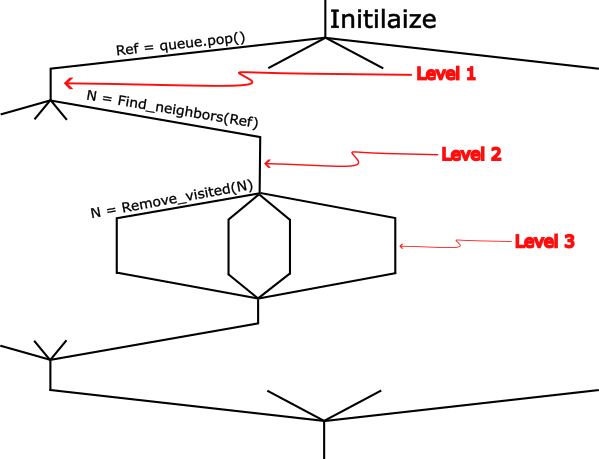
\includegraphics[scale=1.2]{nested.png}
    \caption{Schematic of the nested parallelization used in this work. Only one part of the threading is shown as fully expanded. In this schematic, each parent thread spawns four child threads, but this is arbitrary. The effect of different thread numbers for different levels is investigated here.}
    \label{fig:nested}
    \centering
\end{figure}

\section{Final results and future work}
Firstly, the serial and parallel algorithms are verified by confirming that the hyperlattice matrix, $\mathbf{H}$, obtained from the analysis of a perfect system reproduces the system exactly. The ideal system reproduction is shown in Figure \ref{fig:recontruction}. In testing the parallel computing techniques detailed in the preceding section, variations of the serial algorithm were applied 2 systems: a small system of ~20,000 particles, and a large system of ~100,000 particles. A table of all timed variations is given in Appendix A. In this section, relevant excerpts are presented.

\begin{figure}[htp!]
    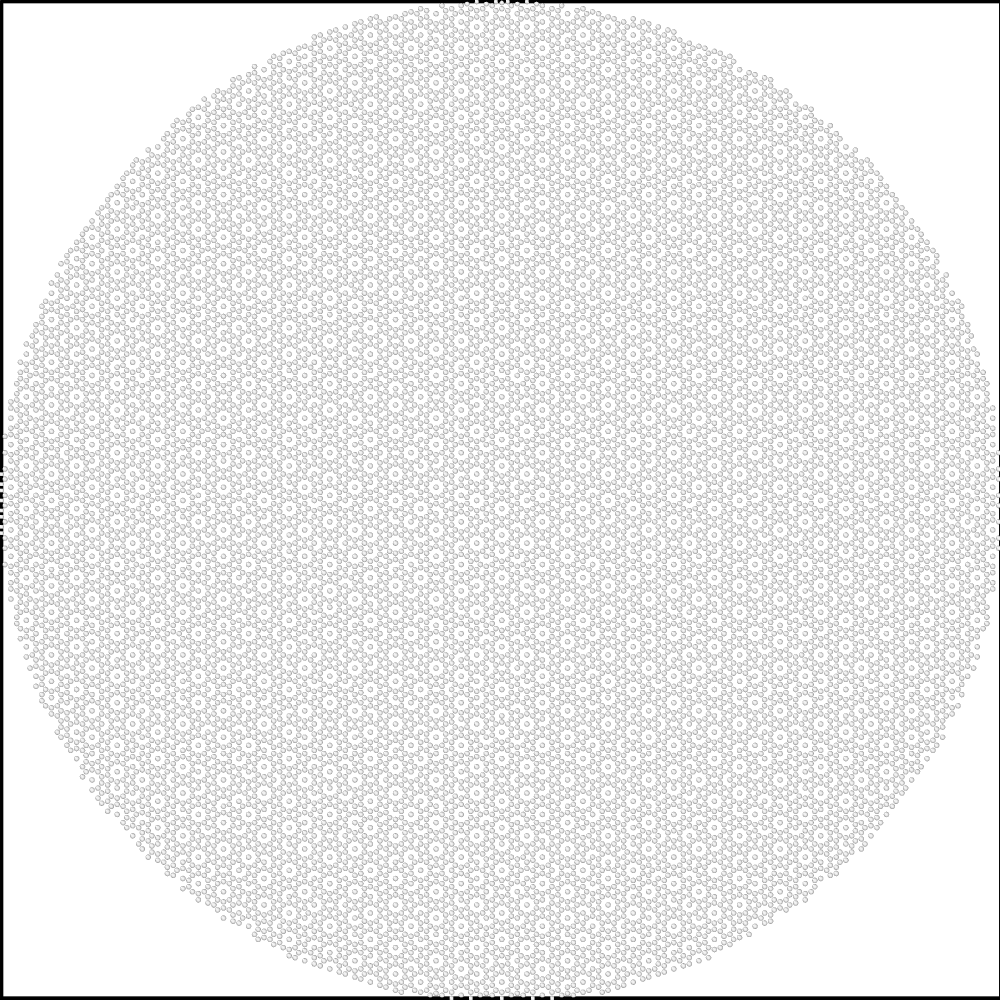
\includegraphics[scale=0.3]{recontruction.png}
    \caption{Verification that the algorithm produces the correct $\mathbf{H}$. The operation $\mathbf{Q^TH^T}$ produces the coordinates for an perfect tiling}
    \label{fig:recontruction}
    \centering
\end{figure}

\subsection{GPU kernelized matrix multiplication}
In most cases, the overhead associated with copying $\mathbf{D}$ and $\mathbf{V}$ to the GPU equates to the benefits gained from a parallelized matrix multiplication. This is likely due to the fact that the matrices are not large enough to benefit from the speed gained from performing operations on the GPU. However, the fact that the costs do not greatly outweigh the benefits suggests that kernelized matrix multiplication may become beneficial for systems in which larger matrices must be multiplied. This include systems which are periodic in even higher number of dimensions (i.e. $\mathbf{Q}$ is larger) and/or denser systems (i.e. $\mathbf{V}$ is larger). 

\subsection{Nested array searching}
The most significant speedup was attained from parallelizing searching the neighbor list array and array of visited particles.
\subsubsection{Neighbor list searching}
Figure \ref{fig:NeighbourSearching} shows how, for both the small and large system, parallelizing the neighbor list search reduces computation time, up to 4 threads. However, when the number of threads is increased to 8, a minor benefit is observed only for the large system. A finer degree of parallelization is therefore expected to benefit systems even larger than the ones that are examined in this work. The speedup for 2 threads is also higher for the large system, than for the small system (1.64 vs. 1.4).  
\begin{figure}[htp!]
    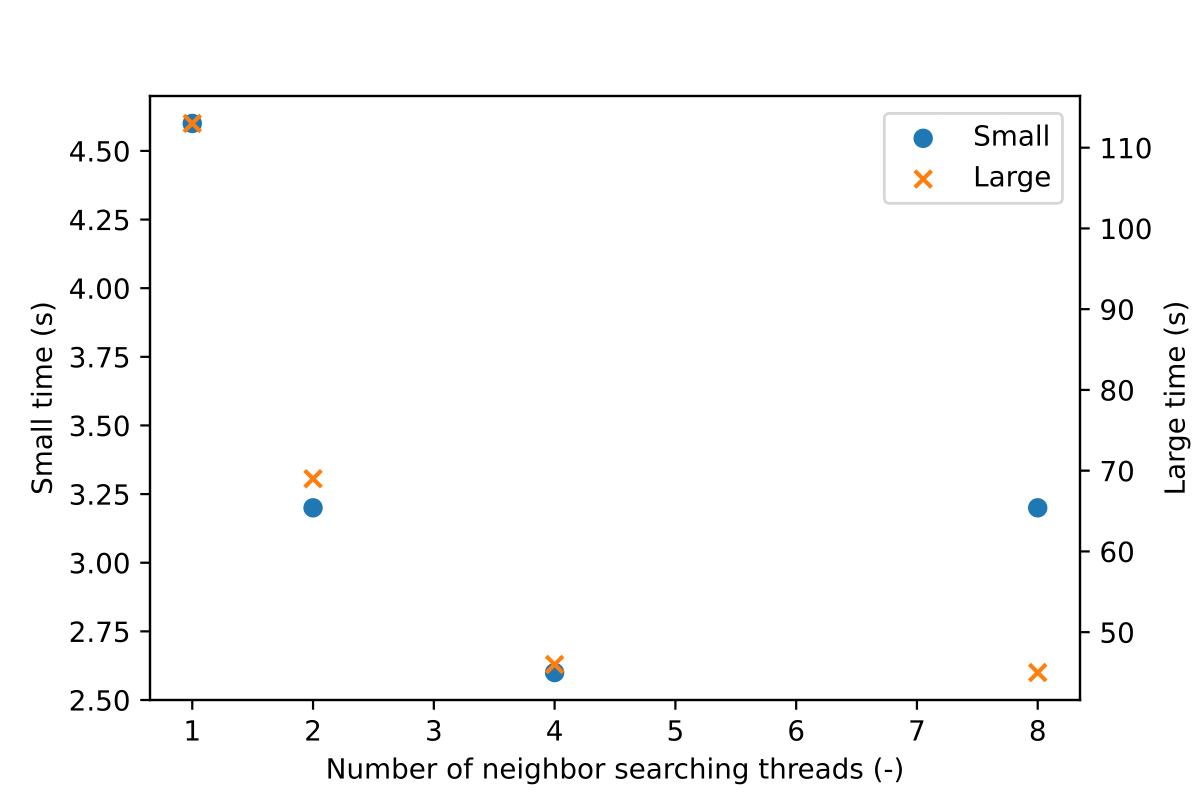
\includegraphics[scale=0.8]{NeighbourSearching.png}
    \caption{Time taken to run the parallel lifting algorithm, as a function of number of threads used in searching the neighbor list, for the small and large system.}
    \centering
    \label{fig:NeighbourSearching}
\end{figure}

\subsubsection{Visitor list searching}
Similar to the preceding section, figure \ref{fig:VisitorSearching} shows how, the benefits from parallelization are greater for the large system. A finer degree of parallelization is therefore expected to benefit systems even larger than the ones that are examined in this work. Interestingly, using 2 threads for searching the neighbor list, and 2 threads for each neighbor list searching thread for visited list searching results in a time of 79 s for the large system.
\begin{figure}[htp!]
    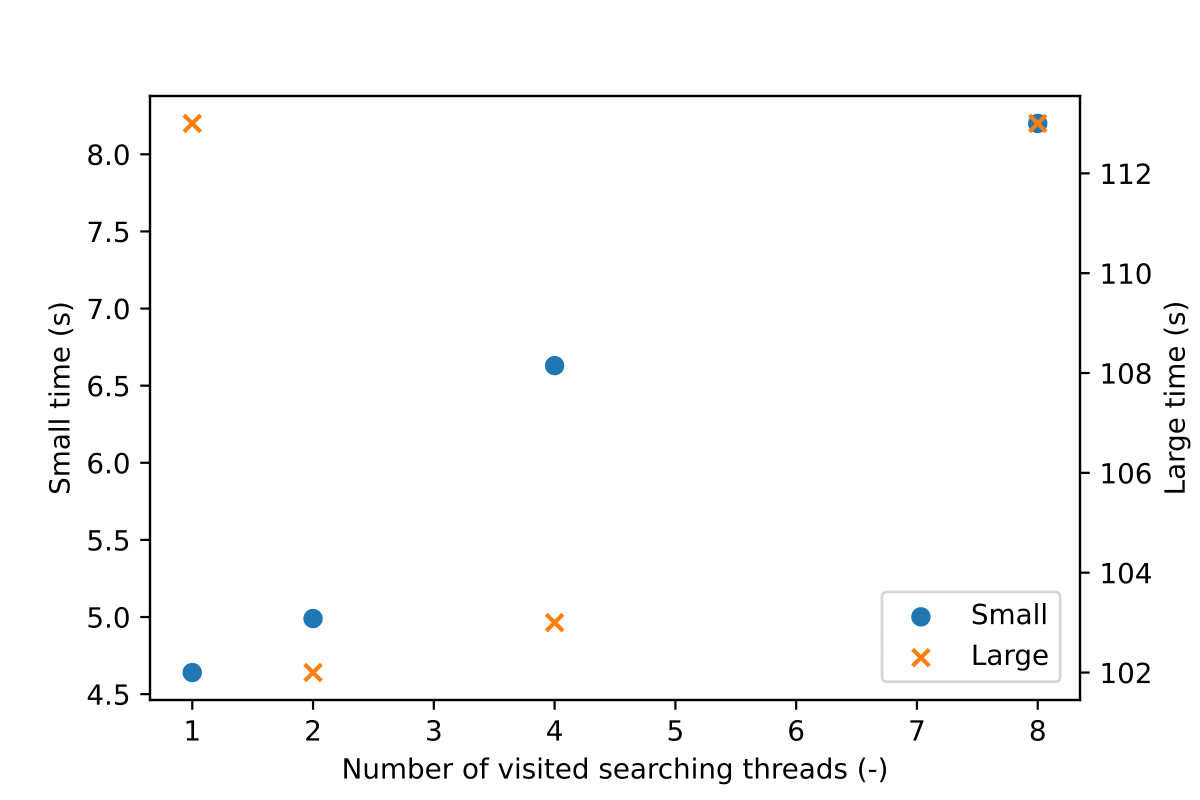
\includegraphics[scale=0.8]{VisitedSearching.png}
    \caption{Time taken to run the parallel lifting algorithm, as a function of number of threads used in searching the visited list, for the small and large system.}
    \centering
    \label{fig:VisitorSearching}
\end{figure}

\section{Discussion and future work}
From analysis of the lifting times for systems examined in this work, it is clear that the system sizes are only just on the cusp of being large enough to benefit from the employed parallelization techniques. Unfortunately, in our research group, larger systems are very difficult to analyze, precisely because our hitherto approach has been a Python implemented serial algorithm, whose inefficiencies have prohibited rapid analysis of systems much larger than 100,000 particles. However, the performance improvement of porting the code to C++ is reason enough to start analyzing larger systems. The current parallelized algorithm will be well poised to benefit even further from the much larger resulting simulations that are currently underway as part of future work. Eventually our group plans to run systems 100x larger than the largest systems examined in this work.

\pagebreak

\section{Appendix A: Complete list of timings}
\begin{figure}[htp!]
    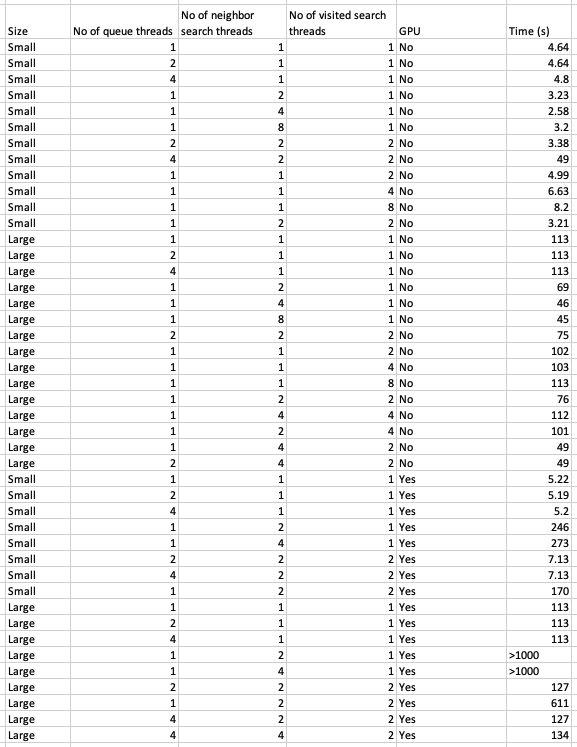
\includegraphics[scale=0.8]{timings.png}
    \caption{Complete list of timings used to assess variations of the parallel lifting algorithm}
    \centering
    \label{fig:recontruction}
\end{figure}

\end{document}